%%%%%%%%%%%%%%%%%%%%%%%%%%%%%%%%%%%%%%%%%%%%%%%%%%%%%%%%%%%%%%%%%%%%%%%%%%%%%%%

\documentclass[12pt,modern,tighten]{aastex63}
%\documentclass[12pt,twocolumn,tighten,linenumbers]{aastex63}
%\documentclass[12pt,twocolumn,tighten,trackchanges]{aastex63}
\usepackage{amsmath,amstext,amssymb}
\usepackage[T1]{fontenc}
\usepackage{apjfonts}
\usepackage[figure,figure*]{hypcap}
\usepackage{graphics,graphicx}
\usepackage{hyperref}
\usepackage{natbib}
\usepackage[caption=false]{subfig} % for subfloat
\usepackage{enumitem} % for specific spacing of enumerate
\usepackage{epigraph}

\renewcommand*{\sectionautorefname}{Section} %for \autoref
\renewcommand*{\subsectionautorefname}{Section} %for \autoref

\newcommand{\cn}{$\delta$~Lyr\ cluster} % cluster name
\newcommand{\sn}{Kepler\,1627} % star system name (binary)
\newcommand{\pn}{Kepler\,1627Ab} % planet name

% gaia target sample numbers
\newcommand{\nkinematic}{3{,}298} % "fullfaint" kinematic sample, core+halo (CG18+KC19+M21). from any call of earhat.helpers._get_fullfaint_dataframes
\newcommand{\nnbhd}{13{,}843} % make_compstar_NGC_2516_sourcelist.py
\newcommand{\ncore}{1{,}106}  % "fullfaint" kinematic sample, CG18. from any call of earhat.helpers._get_fullfaint_dataframes
\newcommand{\nhalo}{2{,}192} % "fullfaint" kinematic sample, KC19+M21. from any call of earhat.helpers._get_fullfaint_dataframes


%
% Symbols
%
\newcommand{\kms}{\,km\,s$^{-1}$}
\newcommand{\ms}{\,m\,s$^{-1}$}
\newcommand{\bpmrpo}{(G_{\rm BP}-G_{\rm RP})_0}
\newcommand{\bpmrp}{G_{\rm BP}-G_{\rm RP}}

%% Reintroduced the \received and \accepted commands from AASTeX v5.2.
%% Add "Submitted to " argument.
\received{---}
\revised{---}
\accepted{---}
\submitjournal{Nature}
\shorttitle{Kepler\,1627}

\begin{document}

\defcitealias{cantatgaudin_gaia_2018}{CG18}
\defcitealias{kounkel_untangling_2019}{KC19}
\defcitealias{meingast_2021}{M21}

% Cluster Difference Imaging Photometric Survey. III.
% Rotation and Lithium in an Open Cluster Spanning 500\,Parsecs
\title{
  An Adolescent Mini-Neptune in the Kepler Field
}

%\suppressAffiliations
%\NewPageAfterKeywords
\correspondingauthor{L.\,G.\,Bouma}
\email{bouma.luke@gmail.com}

\author[0000-0002-0514-5538]{L. G. Bouma}
\affiliation{Department of Astrophysical Sciences, Princeton University, 4 Ivy Lane, Princeton, NJ 08540, USA}

% Key authors:
% ... stellar rotation & the initial crossmatch
\author[0000-0002-2792-134X]{J. L. Curtis}
\affiliation{Department of Astronomy, Columbia University, 550 West 120th Street, New York, NY 10027, USA}
\affiliation{Department of Astrophysics, American Museum of Natural History, New York, NY 10024, USA}

% ... Kepler correlations
\author[0000-0003-1298-9699]{K. Masuda}
\affiliation{Department of Earth and Space Science, Osaka University, Osaka 560-0043, Japan}

% ... HIRES PI
\author{L. A. Hillenbrand}
\affiliation{Cahill Center for Astrophysics, California Institute of Technology, Pasadena, CA 91125, USA}

% ... RM fitting
\author[0000-0001-7409-5688]{G. Stefansson}
\affiliation{Department of Astrophysical Sciences, Princeton University, 4 Ivy Lane, Princeton, NJ 08540, USA}

%
% PFS Collaborators
%
\author[0000-0001-8638-0320]{A. W. Howard}
\affiliation{Cahill Center for Astrophysics, California Institute of Technology, Pasadena, CA 91125, USA}
%
\author[0000-0002-0531-1073]{H. Isaacson}
\affiliation{Astronomy Department, University of California, Berkeley,
CA 94720, USA}

%
% MUSCAT3 Collaborators
%
\author[0000-0001-8511-2981]{N. Narita}
\affiliation{Komaba Institute for Science, The University of Tokyo, Tokyo 153-8902, Japan}
\affiliation{Japan Science and Technology Agency, PRESTO, Tokyo 153-8902, Japan}
\affiliation{Astrobiology Center, Tokyo 181-8588, Japan}
\affiliation{Instituto de Astrof\'{i}sica de Canarias (IAC), 38205 La Laguna, Tenerife, Spain}

\author[0000-0002-4909-5763]{A. Fukui} % afukui@g.ecc.u-tokyo.ac.jp
\affiliation{Komaba Institute for Science, The University of Tokyo, Tokyo 153-8902, Japan}
\affiliation{Instituto de Astrof\'{i}sica de Canarias (IAC), 38205 La Laguna, Tenerife, Spain}

\author[0000-0002-5658-5971]{Masahiro Ikoma} % ikoma.masahiro@gmail.com
\affiliation{Division of Science, National Astronomical Observatory of Japan, Tokyo 181-8588, Japan}

\author[0000-0002-6510-0681]{M. Tamura} % motohide.tamura@nao.ac.jp
\affiliation{Department of Astronomy, University of Tokyo, Tokyo 113-0033, Japan}
\affiliation{Astrobiology Center, Tokyo 181-8588, Japan}
\affiliation{National Astronomical Observatory of Japan, Tokyo 181-8588, Japan}

% AO IMAGING
\author[0000-0001-9800-6248]{E. Furlan} % furlan@ipac.caltech.edu
\affiliation{NASA Exoplanet Science Institute, Caltech/IPAC, Pasadena, CA 91125, USA}

\author[0000-0003-2519-6161]{C.~L.~Gnilka} % clgnilka@gmail.com
\affiliation{NASA Ames Research Center, Moffett Field, CA 94035, USA}

\author[0000-0002-9903-9911]{K.~V.~Lester} % klester192@gmail.com
\affiliation{NASA Ames Research Center, Moffett Field, CA 94035, USA}

\author[0000-0002-2532-2853]{S. B. Howell}
\affiliation{NASA Ames Research Center, Moffett Field, CA 94035, USA}




\begin{abstract}
  Kepler\,1627A is an active G8V star previously found to host a
  $3.6\,R_\oplus$ mini-Neptune on a 7.2\,day orbit.  The star was
  selected for observation by the Kepler satellite because it is
  nearby ($d\approx 333\,{\rm pc}$) and resembles the Sun.  Combining
  data from the Gaia satellite with rotation periods from TESS, we
  show that Kepler\,1627 is a member of the $35\pm 10$\,Myr old
  $\delta$~Lyr cluster.  Our analysis advances Kepler\,1627Ab as the
  youngest planet with a precise age detected by the main Kepler
  mission.  New ages from the combination of Gaia and TESS offer the
  opportunity to significantly expand the census of age-dated planets
  -- we offer a literature concatenation of young stars to support
  this effort.  Future studies of \pn\ may also help clarify how the
  orbits and atmospheres of the mini-Neptune planets evolve.
\end{abstract}

\keywords{
  planetary evolution (XXXX),
  stellar associations (1582),
  open star clusters (1160),
	stellar ages (1581),
}

%%%%%%%%%%%%%%%%%%%%%%%%%%%%%%%%%%%%%%%%%%%%%%%%%%%%%%%%%%%%%%%%%%%%%%%%%%%%%%%


\section{Manuscript}

While thousands of exoplanets have been discovered orbiting nearby
stars, the vast majority of them are several billion years old.  This
results in difficulty testing theories for the origins of the
different families of planets, since many expected evolutionary
processes operate on timescales of less than 100 million years.  

For instance, the ``mini-Neptune'' planets, thought to be made of
molten rocky cores and extended atmospheric envelopes of hydrogen and
helium, are expected to shrink in size by factors of several over
their first $10^8$ years \citep{owen_constraining_2020}.
Specifically, they start with sizes of 4--12\,$R_\oplus$ at the time
of disk dispersal ($\approx$$10^7$\,years), and shrink to sizes of
2--4\,$R_\oplus$ by 10$^8$ years.  This change is driven by a
combination of stellar irradiation and internal heat that powers an
outflow, which eventually depletes or entirely strips the envelope
from the rocky core \citep{Owen_Wu_2013,gupta_sculpting_2019}.
Discovering young planets and measuring their compositions and
atmospheric outflows are key steps toward testing this paradigm, which
is often invoked to explain the observed radius distribution of both
mature exoplanets \citep{Fulton_et_al_2017}, as well as younger
planets \citep{bouma_cluster_2020}.

% The orbits of the planets can also change early on, and can become
% significantly misaligned from the equators of their host stars.
% Measurements of the sky-projected angle between the planet orbit and
% the stellar spin (the stellar obliquity) have shown that high
% obliquities characterize hot field stars hosting both hot Jupiters and
% smaller planets \citep{winn10,louden21}.  Conversely, the obliquities
% of planets around cool stars tend to be low, but this could be due to
% tidal realignment \citep[{\it e.g.},][]{anderson21}.  Obliquity
% measurements for young planets are therefore important, because they
% provide an unobstructed view of the primordial obliquity distribution. 

\begin{figure*}[t]
	\begin{center}
		\leavevmode
		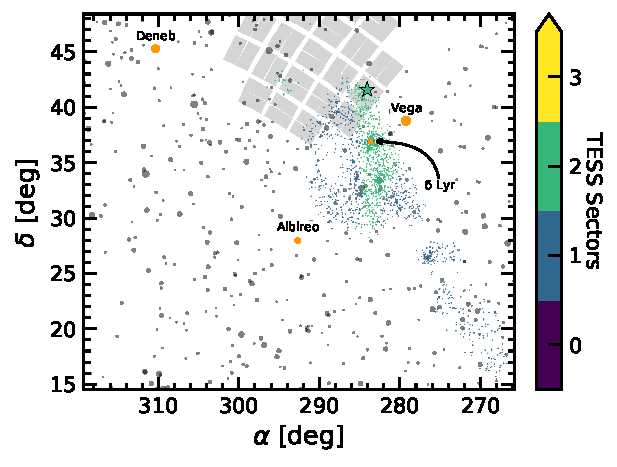
\includegraphics[width=0.99\textwidth]{f2.pdf}
	\end{center}
	\vspace{-0.7cm}
	\caption{
		{\bf Kepler and TESS views of the $\delta$\,Lyr cluster.} Colored
		points are kinematically selected members of the $\delta$\,Lyr
		cluster (black points in Figure~\ref{fig:XYZvtang}).  Both Kepler
		(gray squares) and TESS (colored points) observed portions of the
		cluster.  Naked-eye stars ($m_{\rm V}<6.5$) are shown in gray; four
		of them (orange points) have their names annotated.  Kepler\,1627 (green
		star) was observed during the entirety of the Kepler mission, and
		has been observed  by TESS for two lunar months to date.
		\label{fig:skychart}
	}
\end{figure*}

\begin{figure*}[t]
	\begin{center}
		\leavevmode
		\subfloat{
			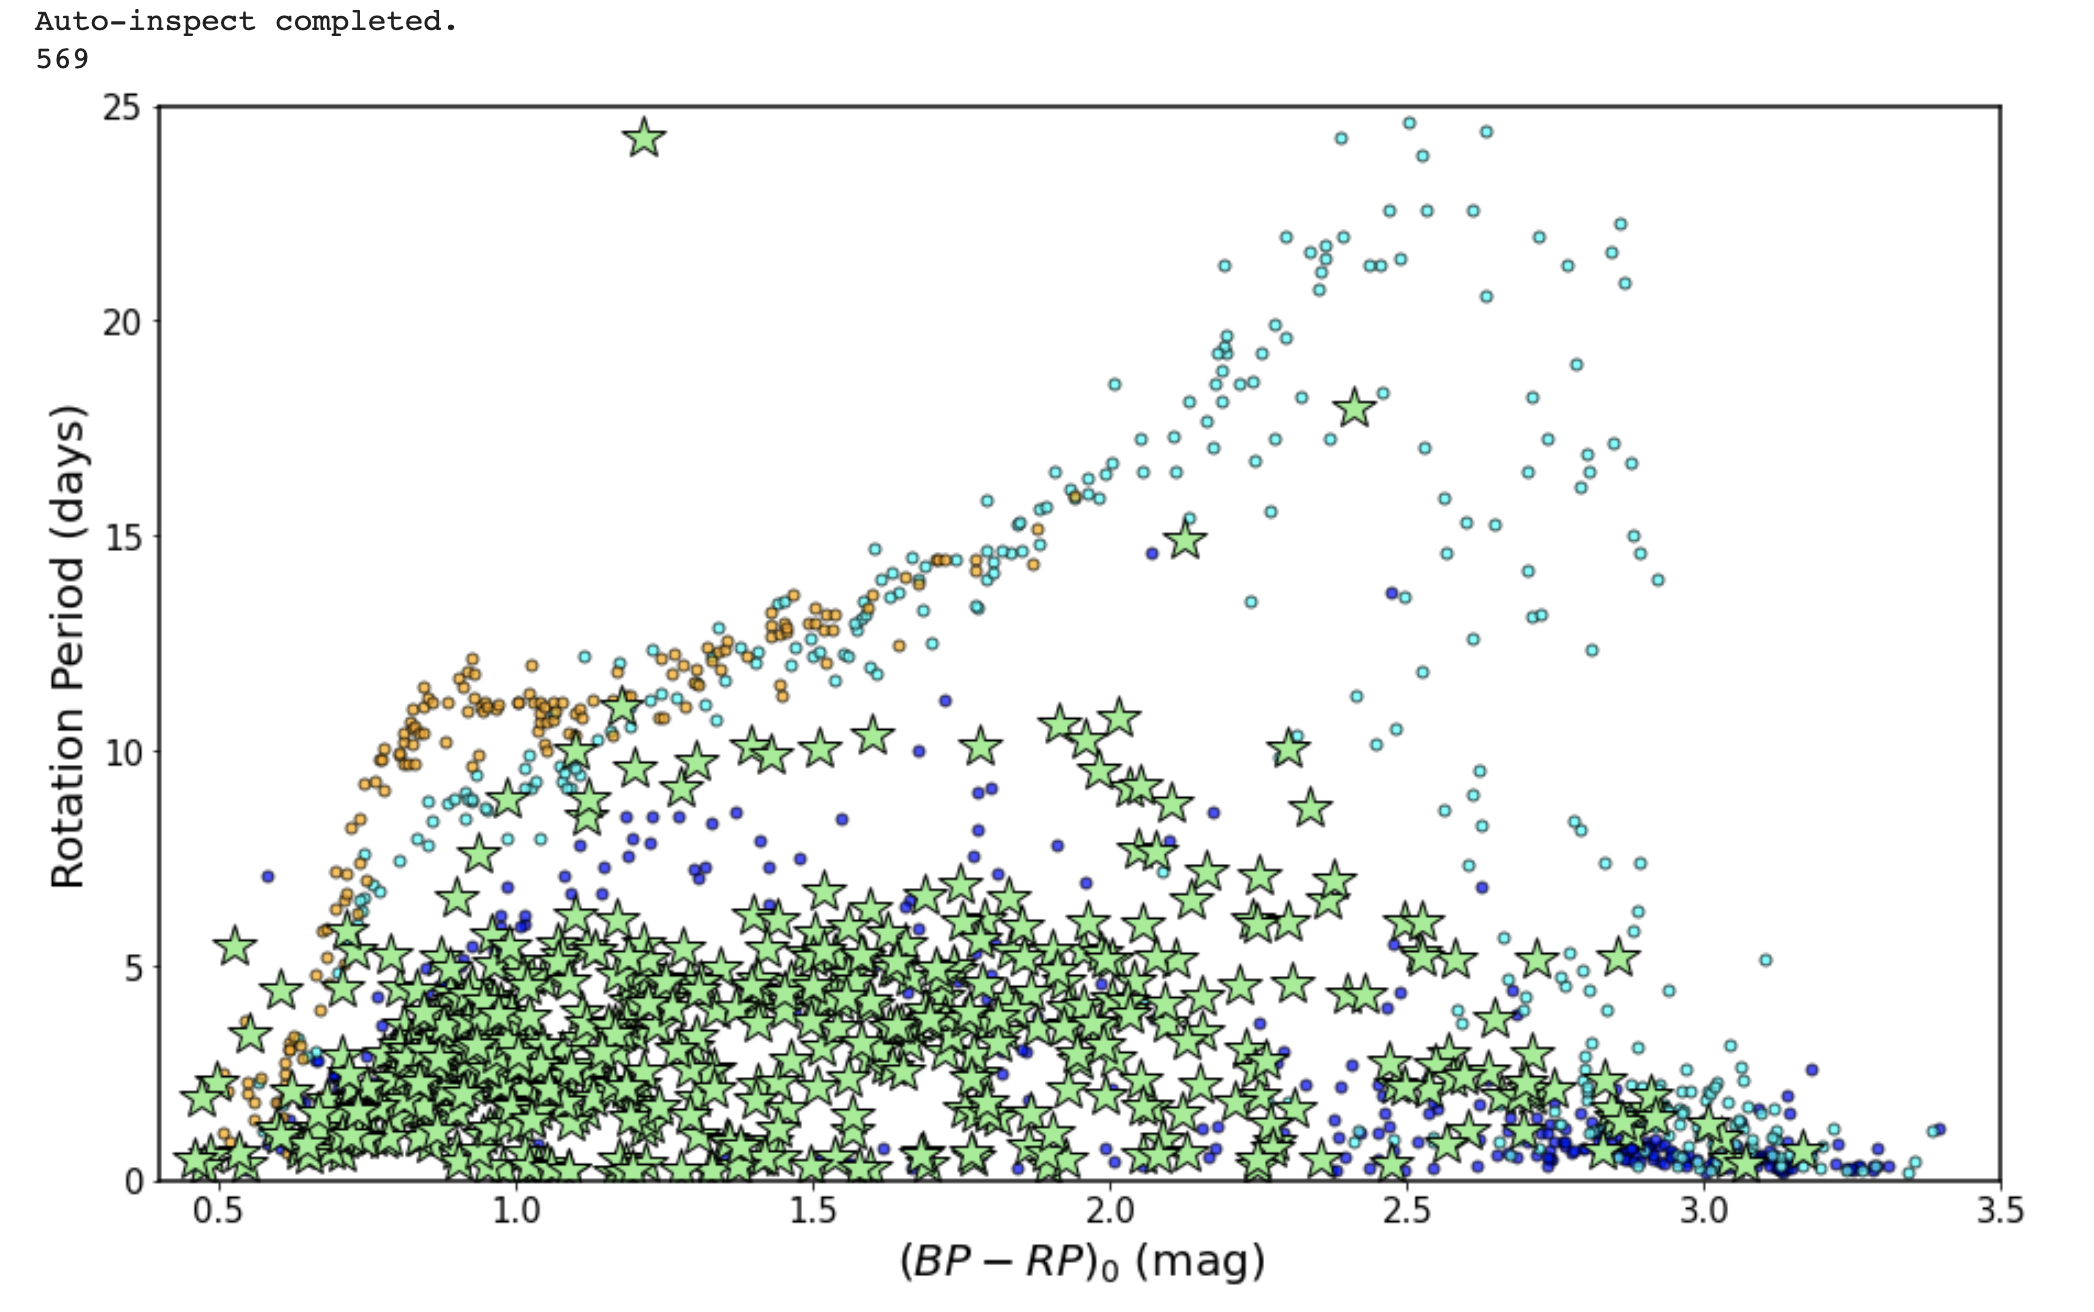
\includegraphics[width=0.49\textwidth]{TEMP_Prot_vs_BpmRp.png}
			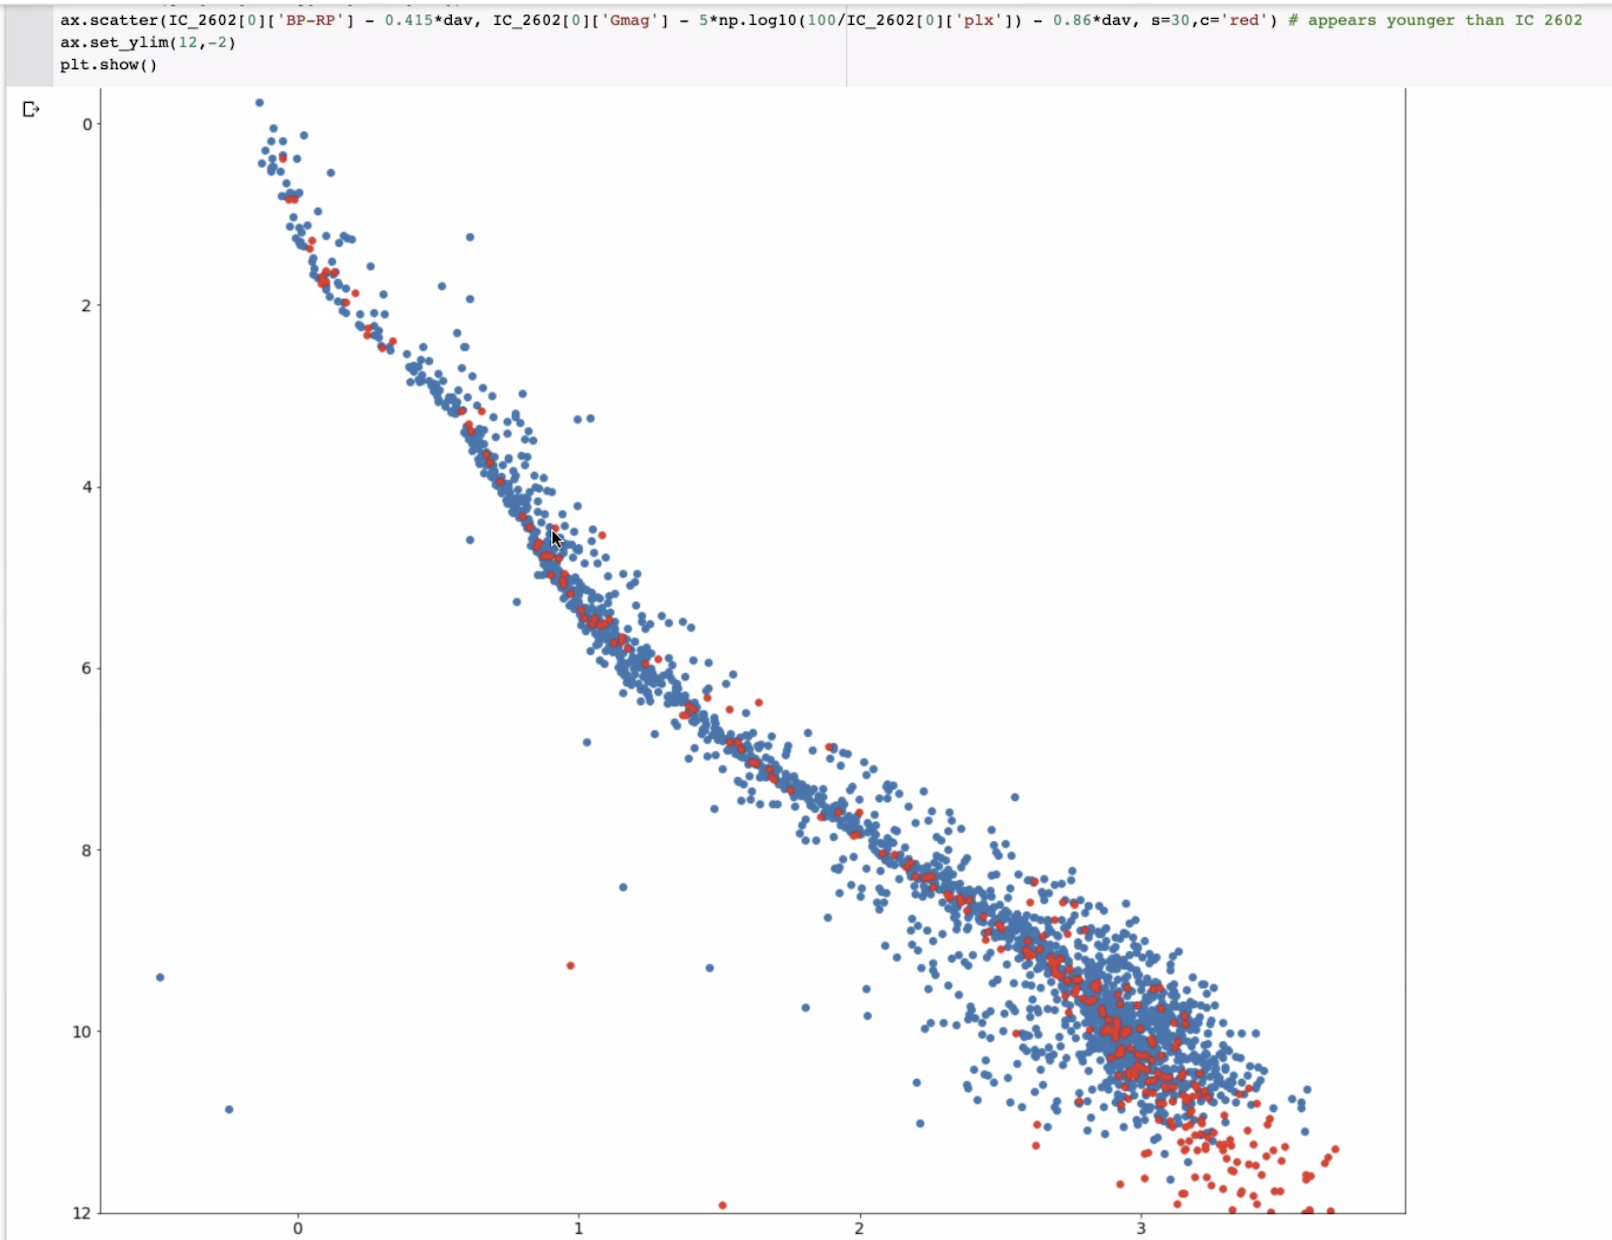
\includegraphics[width=0.49\textwidth]{TEMP_hrd.png}
		}
	\end{center}
	\vspace{-0.7cm}
	\caption{
    {\bf \cn is $35\pm15$\,Myr old.} {\it Left:} TESS and
    Kepler rotations periods and dereddened Gaia colors, with the
    Pleiades \citep[125\,Myr;][]{rebull_rotation_2016a} and Praesepe
    \citep[650\,Myr;][]{douglas_poking_2017} shown for reference.
    Stars of a given color (mass) move up through time due to magnetic
    braking.  The \cn\ has a 40 Myr gyrochronal age, as calibrated
    against the LDB-age of IC\,2602.  {\it Right:} HR diagram of the
    same comparison. {\bf todo: caption improve}.
   \label{fig:age}
	}
\end{figure*}

\begin{figure*}[t]
	\begin{center}
		\leavevmode
		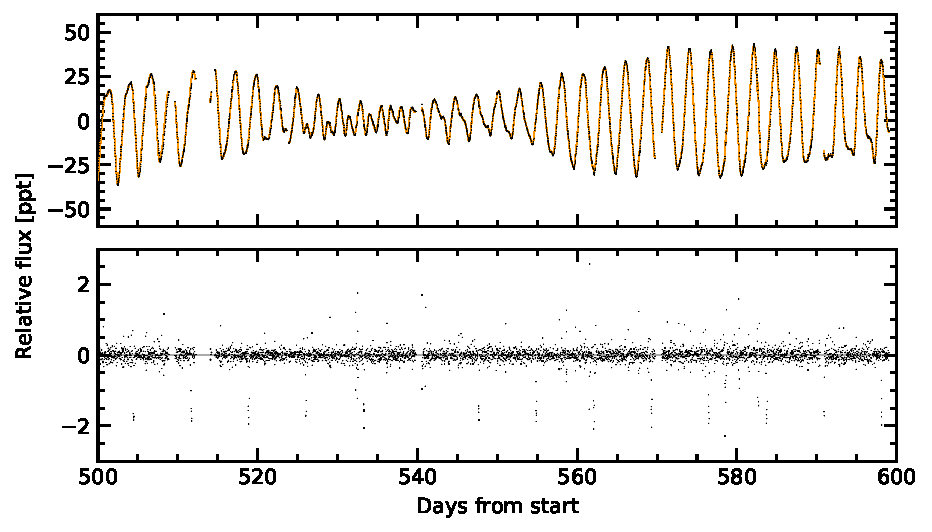
\includegraphics[width=1\textwidth]{f4.pdf}
	\end{center}
	\vspace{-0.7cm}
	\caption{
		{\bf Zoomed view of the \sn\ light curve.}  
		The full Kepler dataset spans 1{,}437 days (3.9 years), sampled at
		30 minute cadence.  A one hundred day segment is shown here.  The {\it top panel} shows the
		\texttt{PDCSAP} median-subtracted flux in units of
		parts-per-thousand ($\times 10^{-3}$).  The dominant signal
		is induced by starspots and plages.  The model for the
		stellar variability (orange line) is subtracted in the {\it
			bottom panel}, revealing the transits of \pn, as well as other
		deviations from the stellar variability model.  The 
		Figure Set available online shows the entire 3.9 years of
		available data.
		\label{fig:lightcurve}
	}
\end{figure*}

\begin{figure*}[t]
	\begin{center}
		\leavevmode
		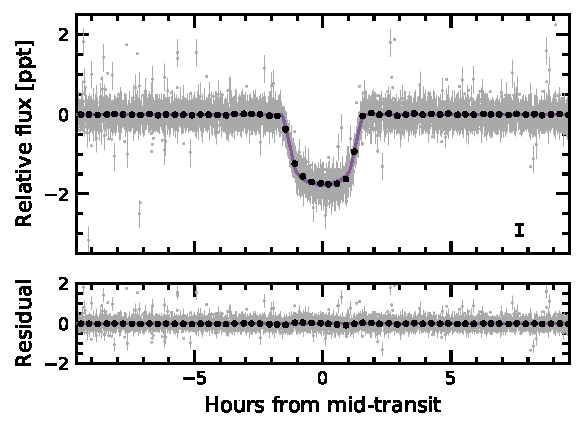
\includegraphics[width=1\textwidth]{f5.pdf}
	\end{center}
	\vspace{-0.7cm}
	\caption{
		{\bf Phase-folded transit of Kepler 1627b, with stellar
			variability removed.}  
    The 1-$\sigma$ model uncertainties and the maximum {\it a
    posteriori} model are shown as the faint purple band, and the dark
    purple line.  Gray points are individual \texttt{PDCSAP} flux
    measurements; black points are binned to 20 minutes, with a
    representative error bar shown.
    {\bf LGB FIXME: seems like the uncertainty is bigger than the RMS
    in the out of transit...}
		\label{fig:phasefold}
	}
\end{figure*}

At the time of the main Kepler mission (2009--2013), only four open
clusters were known in the Kepler field: NGC\,6866, NGC\,6811,
NGC\,6819, and NGC\,6791, with ages spanning 0.7\,Gyr to 9\,Gyr
\citep{meibom_kepler_2011}.  Since that time, analyses of the
kinematic, photometric, and astrometric Gaia data have expanded our
knowledge of open cluster and moving group memberships \citep[{\it
e.g.},][]{cantatgaudin_gaia_2018,zari_3d_2018,kounkel_untangling_2019,Meingast2021}.
As part of our Cluster Difference Imaging Photometric Survey (CDIPS,
\citealt{bouma_cdipsI_2019}), we concatenated the available analyses
from the literature, which yielded a list of candidate young and
age-dated stars (see Section~\ref{app:targetlist}).

Comparing our young star list against the Kepler field yielded two
discoveries.  The first, to be discussed in an upcoming analysis
by J. Curtis et al{.}, is that Kepler observed the $\approx$350\,Myr
open cluster Theia\,520 (UBC\,1).  At least five Kepler planets are
known in the cluster, including the Kepler-52 and Kepler-968 systems.
The second discovery, and the focus of this work, is that Kepler
observed a portion of the $\delta$\,Lyr cluster, shown in
Figure~\ref{fig:skychart}.

While we have yet to perform an in-depth planet search of the {\bf
XXX} light curves Kepler acquired for the \cn, there is already a
known planet in the cluster: Kepler\,1627b.  We considered the
planet's previous statistical validation by \citet{morton_false_2016}
to be sufficient cause to examine the age of the star and its cluster more closely.
We collected the previously measured {\bf XXX} Kepler
rotation periods (CITEP MCQUILLAN2014), and measured {\bf YYY} new stellar
rotation periods for cluster members observed by TESS.
We also performed an isochronal analysis.
The results are shown in Figure~\ref{fig:age}.
From the ensemble perspective, which provides the strongest
constraints (SEE CITET SODERBLOM 2014),
the age of the star is $XX \pm YY$\,Myr.
Individual measurements of the star's rotation period and lithium
abundance corroborate this conclusion.

If the Kepler\,1627b transit signal truly corresponds to a planet,
this age would make it the youngest planet yet found by the main
Kepler mission.  A portion of the light curve is shown in
Figure~\ref{fig:lightcurve}, and the phase-folded transit is shown in
Figure~\ref{fig:phasefold}.  The dominant signal in the
\texttt{PDCSAP} photometry is a quasi-period starspot signal with a
peak-to-peak amplitude that varies between roughly 2\% and 8\%,
depending on the degree of asymmetry in spot coverage between the
stellar hemispheres.  The starspot signal repeats roughly every
2.606\,days, though this value varies by a few percent depending on
which portion of the light curve is analyzed {\bf (FIXME: do!)}.  The
details of how we model this signal to derive the parameters of the
planet are discussed in Section~\ref{app:gptransit}.  The results,
given in Table~\ref{tab:posterior}, are consistent with a mini-Neptune
sized planet ($3.56\pm 0.04\,R_\oplus$) on a circular 7.2\,day orbit,
around a G8V star ($0.91 \pm 0.05 R_\odot$) {\bf fixme: age}. 

Could the transit signal be produced by anything other than a planet
orbiting this near-solar analog?  \citet{morton_false_2016} considered
the various false positive scenarios, including those of a foreground
eclipsing binary, a hierarchical triple-star binary system, and a
background eclipsing binary.  \citet{morton_false_2016} reported the
latter scenario to be the only possible case, with a (model-dependent)
probability of $\approx10^{-5}$.  While this statistical validation is
reassuring, ``validated'' planets have been demonstrated to be false
positives \citep{shporer_three_2017}.  Most failures of the
statistical validation approach arise when attempting to separate the
smallest stars from identically-sized gas giant planets (CITE).  With a size
of $\approx 3.6\,R_\oplus$, Kepler\,1627b does not meet this
concern.  The fact that we detect a low-mass stellar companion in
archival Keck-NIRC2 Kp-band (2.12\,$\mu $m) imaging does not change
the conclusion: the companion contributes 1\% of the flux
observed by Kepler, which combined with the observed transit shape
cannot be invoked as an explanation for the observed data
(Section~\ref{app:companionstar}).

% Could the planet be on a high obliquity orbit?
% * how do the spectroscopic vsini and the measured v_rot=2πRstar/Prot compare?
%   * Rstar=0.91+-0.05, 2.606 days gives vsini=17.6km/s (+/-0.97km/s)
% * spectroscopic vsini is 18.8 +/- 4.7km/s from Keck HIRES... "20km/s" from
%   TRES.


Kepler\,1627Ab therefore provides an interesting extremum in the ages
of the Kepler planets, and opens multiple avenues for study from the
ground.  Observations of its Doppler transit ($\Delta v_{\rm RM}
\approx 20$\ms) with HIRES or the upcoming KPF spectrograph could
yield a measurement of its orbital obliquity (CITEP,CITEP).
Similarly, transit spectroscopy aimed at detecting either hydrogen or
helium absorption could yield insight into the planet's atmosphere,
which is expected to be outflowing at a rate of {\bf
X.X}\,$M_\oplus\,{\rm yr}^{-1}$ (CITE).  A more challenging
measurement would be a measurement of the planet's mass, through
either detailed timing analyses of the Kepler data, or through a
high-cadence multi-color radial velocity campaign.  The mass would
yield constraints on both the planet's composition (``what is the
extent of the initial gaseous envelope for a typical mini-Neptune?''),
as well as its initial entropy (``hot'' or ``cold''? CITE).

The precision of the Kepler data itself may enable more detailed
analyses without even needing to acquire more data.  These could
include studies transit timing variations, distortion of the transit
signal due to the star's gravity darkening, and interactions between
the star and planet exhibited by patterns in the star's flaring.
The gravity darkening might be interesting as an explanation for the
$\approx80\,{\rm ppm}$ residual apparent in our transit fit.
On the point of planet-induced flaring, Appendix REFERENCE
highlights an odd timing coincidence that may be worthy of further
examination.  

Ultimately though, our age measurement for Kepler\,6127Ab was enabled by
identifying its connection to the \cn\ through the Gaia data.  The
Supplementary Table~\ref{tab:v05} enables similar crossmatches to
already known planets, as well as forthcoming planets from the TESS
mission (CITE RickerJATIS2014).  An alternative approach also
likely to bear fruit is to identify kinematic associations
around exoplanet host stars using the Gaia data, and to then verify
these associations with ancilliary rotation periods and spectroscopy
(CITEP Tofflemire).


%%%%%%%%%%%%%%%%%%%%%%%%%%%%%%%%%%%%%%%%%%%%%%%%%%%%%%%%%%%%%%%%%%%%%%%%%%%%%%%



% Table of best fit parameters
%\startlongtable
\begin{deluxetable*}{lllrrrrrrr}
%
  \tablecaption{ Priors and posteriors for the transit and stellar
  variability model fitted to the long-cadence Kepler 1627b
  photometric timeseries.}
\label{tab:posterior}
%
\tabletypesize{\scriptsize}
%\tabletypesize{\small}
%
%\tablenum{2}
%
\tablehead{
  \colhead{Param.} & 
  \colhead{Unit} &
  \colhead{Prior} & 
  \colhead{Median} & 
  \colhead{Mean} & 
  \colhead{Std{.} Dev.} &
  \colhead{3\%} &
  \colhead{97\%} &
  \colhead{ESS} &
  \colhead{$\hat{R}-1$}
}

%/Users/luke/Dropbox/proj/rudolf/results/run_RotStochGPtransit/Kepler_1627_RotStochGPtransit_posteriortable.tex
\startdata
{\it Sampled} & & & & & & & & & \\
\hline
$P$ & d & $\mathcal{N}(7.20281; 0.01000)$ & 7.2028035 & 7.2028033 & 0.0000073 & 7.2027893 & 7.2028171 & 1910.5903732 & 0.0035905 \\
$t_0^{(1)}$ & d & $\mathcal{N}(120.79053; 0.02000)$ & 120.790504 & 120.790505 & 0.0009438 & 120.7886867 & 120.7922431 & 1564.1105056 & 0.0003213 \\
$\log R_{\rm p}/R_\star$ & -- & $\mathcal{U}(-4.605; 0.000)$ & -3.33523 & -3.33569 & 0.06618 & -3.45772 & -3.21617 & 1173.56574 & 0.00310 \\
$b$ & -- & $\mathcal{U}(0; 1+R_{\mathrm{p}}/R_\star)$ & 0.3971 & 0.3886 & 0.2070 & 0.0204 & 0.7289 & 378.9528 & 0.0177 \\
$u_1$ & -- & \citet{exoplanet:kipping13} & 0.28 & 0.30 & 0.179 & 0.002 & 0.603 & 1161.95 & 0.005 \\
$u_2$ & -- & \citet{exoplanet:kipping13} & 0.425 & 0.381 & 0.314 & -0.197 & 0.912 & 900.884 & 0.002 \\
$R_\star$ & $R_\odot$ & $\mathcal{T}(0.910; 0.052)$ & 0.911 & 0.910 & 0.051 & 0.814 & 1.004 & 2265.830 & -0.001 \\
$\log g$ & cgs & $\mathcal{N}(4.600; 0.100)$ & 4.604 & 4.601 & 0.094 & 4.417 & 4.769 & 923.943 & 0. \\
$\langle f \rangle$ & -- & $\mathcal{N}(0.500; 0.100)$ & 0.4999 & 0.4999 & 0.0003 & 0.4993 & 0.5005 & 2964.6676 & 0.0013 \\
$e^{(2)}$ & -- & \citet{vaneylen19} & 0.127 & 0.168 & 0.147 & 0. & 0.446 & 518.492 & 0.004 \\
$\omega$ & rad & $\mathcal{U}(0.000; 6.283)$ & -0.235 & -0.170 & 1.867 & -2.879 & 3.132 & 1212.260 & 0.006 \\
$\log \sigma_f$ & -- & $\mathcal{N}(\log\langle \sigma_f \rangle; 2.000)$ & -8.016 & -8.016 & 0.008 & -8.031 & -8.001 & 2224.427 & -0. \\
$\rho$ & d & $\mathcal{U}(1.000; 10.000)$ & 2.953 & 2.955 & 0.096 & 2.777 & 3.131 & 1936.492 & 0. \\
$\sigma$ & d$^{-1}$ & $\mathrm{InvGamma}(1.000; 5.000)$ & 0.013 & 0.013 & 0.001 & 0.012 & 0.014 & 2155.687 & -0. \\
$\sigma_{\mathrm{rot}}$ & d$^{-1}$ & $\mathrm{InvGamma}(1.000; 5.000)$ & 0.897 & 0.933 & 0.222 & 0.552 & 1.316 & 2147.324 & 0.003 \\
$\log P_{\mathrm{rot}}$ & $\log (\mathrm{d})$ & $\mathcal{N}(0.958; 0.020)$ & 0.964 & 0.964 & 0.001 & 0.963 & 0.966 & 2486.029 & 0. \\
$\log Q_0$ & -- & $\mathcal{N}(0.000; 2.000)$ & 12.935 & 12.960 & 0.454 & 12.157 & 13.857 & 2126.581 & 0.004 \\
$\log \mathrm{d}Q$ & -- & $\mathcal{N}(0.000; 2.000)$ & 0.029 & 0.021 & 2.032 & -3.785 & 3.780 & 1755.941 & 0. \\
$f$ & -- & $\mathcal{U}(0.100; 1.000)$ & 0.111 & 0.113 & 0.010 & 0.1 & 0.130 & 1253.358 & -0.0 \\
\hline
{\it Derived} & & & & & & & & & \\
\hline
$R_{\rm p}/R_\star$ & -- & -- & 0.036 & 0.036 & 0.002 & 0.031 & 0.040 & 1173.566 & 0.003 \\
$\rho_\star$ & g$\ $cm$^{-3}$ & -- & 2.27 & 2.312 & 0.516 & 1.408 & 3.272 & 910.746 & 0.001 \\
$R_{\rm p}$ & $R_{\mathrm{Jup}}$ & -- & 0.316 & 0.317 & 0.037 & 0.251 & 0.386 & 1692.736 & 0.001 \\
$a/R_\star$ & -- & -- & 18.396 & 18.407 & 1.375 & 15.690 & 20.780 & 910.717 & 0.001 \\
$\cos i$ & -- & -- & 0.022 & 0.021 & 0.011 & 0.002 & 0.038 & 439.303 & 0.011 \\
$T_{14}$ & hr & -- & 2.822 & 2.823 & 0.057 & 2.710 & 2.917 & 1086.008 & 0.002 \\
$T_{13}$ & hr & -- & 2.578 & 2.566 & 0.083 & 2.430 & 2.714 & 590.630 & 0.011 \\
\enddata
%
\tablecomments{
  ESS refers to the number of effective samples.
  $\hat{R}$ is the Gelman-Rubin convergence diagnostic.
  Logarithms through this table are in base-$e$.
  $\mathcal{U}$ denotes a uniform distribution,
  $\mathcal{N}$ a normal distribution, and
  $\mathcal{T}$ a truncated normal bounded between zero and an upper limit much larger than the mean.
  (1) The ephemeris is in units of BJDTDB - 2454833.
  (2) The eccentricity vectors are sampled in the $(e\cos\omega,
  e\sin\omega)$ basis.
%
% (2) Uninformative quadratic limb-darkening prior from \citet{exoplanet:kipping13}, implemented by \citet{exoplanet:exoplanet}.
% The precision achieved in the ground-based data did not appear to
% necessitate using bandpass-dependent limb-darkening coefficients.
% For comparison, the \citet{claret_limb_2017} parameters for
% the appropriate $T_{\rm eff}$ and $\log g$ in TESS-band would have been 
% $(u_1, u_2) = (0.3249, 0.235)$.
%
% (2) Assuming an informative quadratic limb-darkening prior with
% values about those given for the appropriate $T_{\rm eff}$ and
% $\log g$ in TESS-band from \citet{claret_limb_2017}. The precision
% achieved in the ground-based data did not appear to necessitate using
% bandpass-dependent limb-darkening coefficients.
% (3) The second and third contact points do not exist for a grazing transit.
% {\it Notation}:
% $a_{ij;\mathrm{Instr}}$ denotes the $i^{\rm th}$ transit of a
% particular instrument, and the $j^{\rm th}$ polynomial detrending
% order.
}
\vspace{-0.3cm}
\end{deluxetable*}



%\clearpage
\acknowledgements
\raggedbottom

L.G.B{.} and J.L.C{.} are grateful to T{.}~David for help with the
transit fitting, and to R{.}~Kerr for kindly providing us with the
\citet{Kerr2021} membership list prior to its publication.
% is grateful to G.~Zhou, B{.}~Tofflemire, A{.}~McWilliam,
% E{.}~Newton, M{.}~Kounkel, A{.}~Kraus, L{.}~Hillenbrand, and
% K{.}~Hawkins for the discussions on young stars, rotation, and lithium
% that encouraged this analysis.
%
L.G.B{.} acknowledges support by the TESS GI Program, programs
G011103 and G022117, through NASA grants 80NSSC19K0386 and
80NSSC19K1728.
%
L.G.B{.} was also supported by a Charlotte Elizabeth Procter
Fellowship from Princeton University.
%
This study was based in part on observations at Cerro Tololo
Inter-American Observatory at NSF's NOIRLab (NOIRLab Prop{.} ID
2020A-0146; 2020B-0029 PI: Bouma), which is managed by the
Association of Universities for Research in Astronomy (AURA) under a
cooperative agreement with the National Science Foundation.
%
% ACKNOWLEDGE PFS / CAMPANAS.
%
This paper also includes data collected by the TESS mission, which are
publicly available from the Mikulski Archive for Space Telescopes
(MAST).
%
Funding for the TESS mission is provided by NASA's Science Mission
directorate.
%
We thank the TESS Architects (G.~Ricker, R.~Vanderspek, D.~Latham,
S.~Seager, J.~Jenkins) and the many TESS team members for their
efforts to make the mission a continued success.
%

%
% The Digitized Sky Survey was produced at the Space Telescope Science
% Institute under U.S. Government grant NAG W-2166.
% Figure~\ref{fig:scene} is based on photographic data obtained using
% the Oschin Schmidt Telescope on Palomar Mountain.
%

% %
% This research made use of the NASA Exoplanet Archive, which is
% operated by the California Institute of Technology, under contract
% with the National Aeronautics and Space Administration under the
% Exoplanet Exploration Program.
% %

% Resources supporting this work were provided by the NASA High-End
% Computing (HEC) Program through the NASA Advanced Supercomputing (NAS)
% Division at Ames Research Center for the production of the SPOC data
% products.
%

% A.J.\ and R.B.\ acknowledge support from project IC120009 ``Millennium
% Institute of Astrophysics (MAS)'' of the Millenium Science Initiative,
% Chilean Ministry of Economy. A.J.\ acknowledges additional support
% from FONDECYT project 1171208.  J.I.V\ acknowledges support from
% CONICYT-PFCHA/Doctorado Nacional-21191829.  R.B.\ acknowledges support
% from FONDECYT Post-doctoral Fellowship Project 3180246.
% %
% C.T.\ and C.B\ acknowledge support from Australian Research Council
% grants LE150100087, LE160100014, LE180100165, DP170103491 and
% DP190103688.
% %
% C.Z.\ is supported by a Dunlap Fellowship at the Dunlap Institute for
% Astronomy \& Astrophysics, funded through an endowment established by
% the Dunlap family and the University of Toronto.
% %
% D.D.\ acknowledges support through the TESS Guest Investigator Program
% Grant 80NSSC19K1727.
%
%
%
% %
% Based on observations obtained at the Gemini Observatory, which is
% operated by the Association of Universities for Research in Astronomy,
% Inc., under a cooperative agreement with the NSF on behalf of the
% Gemini partnership: the National Science Foundation (United States),
% National Research Council (Canada), CONICYT (Chile), Ministerio de
% Ciencia, Tecnolog\'{i}a e Innovaci\'{o}n Productiva (Argentina),
% Minist\'{e}rio da Ci\^{e}ncia, Tecnologia e Inova\c{c}\~{a}o (Brazil),
% and Korea Astronomy and Space Science Institute (Republic of Korea).
% %
% Observations in the paper made use of the High-Resolution Imaging
% instrument Zorro at Gemini-South. Zorro was funded by the NASA
% Exoplanet Exploration Program and built at the NASA Ames Research
% Center by Steve B. Howell, Nic Scott, Elliott P. Horch, and Emmett
% Quigley.
% %
% This research has made use of the VizieR catalogue access tool, CDS,
% Strasbourg, France. The original description of the VizieR service was
% published in A\&AS 143, 23.
% %
% This work has made use of data from the European Space Agency (ESA)
% mission {\it Gaia} (\url{https://www.cosmos.esa.int/gaia}), processed
% by the {\it Gaia} Data Processing and Analysis Consortium (DPAC,
% \url{https://www.cosmos.esa.int/web/gaia/dpac/consortium}). Funding
% for the DPAC has been provided by national institutions, in particular
% the institutions participating in the {\it Gaia} Multilateral
% Agreement.
%
% (Some of) The data presented herein were obtained at the W. M. Keck
% Observatory, which is operated as a scientific partnership among the
% California Institute of Technology, the University of California and
% the National Aeronautics and Space Administration. The Observatory was
% made possible by the generous financial support of the W. M. Keck
% Foundation.
% The authors wish to recognize and acknowledge the very significant
% cultural role and reverence that the summit of Maunakea has always had
% within the indigenous Hawaiian community.  We are most fortunate to
% have the opportunity to conduct observations from this mountain.
%
% \newline
%

\software{
  %\texttt{arviz} \citep{arviz_2019},
  \texttt{astrobase} \citep{bhatti_astrobase_2018},
  %\texttt{astroplan} \citep{astroplan2018},
	%\texttt{AstroImageJ} \citep{collins_astroimagej_2017},
  \texttt{astropy} \citep{astropy_2018},
  \texttt{astroquery} \citep{astroquery_2018},
  %\texttt{BATMAN} \citep{kreidberg_batman_2015},
  %\texttt{ceres} \citep{brahm_2017_ceres},
  %\texttt{cdips-pipeline} \citep{bhatti_cdips-pipeline_2019},
  \texttt{corner} \citep{corner_2016},
  %\texttt{emcee} \citep{foreman-mackey_emcee_2013},
  \texttt{exoplanet} \citep{exoplanet:exoplanet}, and its
  dependencies \citep{exoplanet:agol20, exoplanet:kipping13, exoplanet:luger18,
   	exoplanet:theano},
	%\texttt{gala} \citep{gala,PriceWhelan_2017_gala_zenodo},
	%\texttt{IDL Astronomy User's Library} \citep{landsman_1995},
  \texttt{IPython} \citep{perez_2007},
	%\texttt{isochrones} \citep{morton_2015_isochrones},
	%\texttt{lightkurve} \citep{lightkurve_2018},
  \texttt{matplotlib} \citep{hunter_matplotlib_2007}, 
  %\texttt{MESA} \citep{paxton_modules_2011,paxton_modules_2013,paxton_modules_2015}
  \texttt{numpy} \citep{walt_numpy_2011}, 
  \texttt{pandas} \citep{mckinney-proc-scipy-2010},
  %\texttt{pyGAM} \citep{serven_pygam_2018_1476122},
  \texttt{PyMC3} \citep{salvatier_2016_PyMC3},
  %\texttt{radvel} \citep{fulton_radvel_2018},
  %\texttt{scikit-learn} \citep{scikit-learn},
  \texttt{scipy} \citep{jones_scipy_2001},
  \texttt{TESS-point}  \citep{burke_2020},
  %\texttt{tesscut} \citep{brasseur_astrocut_2019},
	%\texttt{VESPA} \citep{morton_efficient_2012,vespa_2015},
  %\texttt{webplotdigitzer} \citep{rohatgi_2019},
  \texttt{wotan} \citep{hippke_wotan_2019}.
}
\ 

\facilities{
 	{\it Astrometry}:
 	Gaia \citep{gaia_collaboration_gaia_2018,gaia_collaboration_2020_edr3}.
 	{\it Imaging}:
    Second Generation Digitized Sky Survey. %,
    %SOAR~(HRCam; \citealt{tokovinin_ten_2018}).
 	%Keck:II~(NIRC2; \url{www2.keck.hawaii.edu/inst/nirc2}).
 	%Gemini:South~(Zorro; \citealt{scott_nessi_2018}.
 	{\it Spectroscopy}:
	CTIO1.5$\,$m~(CHIRON; \citealt{tokovinin_chironfiber_2013}),
  %PFS ({\bf CITE}),
  %  MPG2.2$\,$m~(FEROS; \citealt{kaufer_commissioning_1999}),
	%AAT~(Veloce; \citealt{gilbert_veloce_2018}).
	AAT~(HERMES; \citealt{lewis_2002_hermers_2df,sheinis_2015_hermes}),
 	%Keck:I~(HIRES; \citealt{vogt_hires_1994}).
 	VLT:Kueyen~(FLAMES; \citealt{pasquini_2002}).
% 	Euler1.2m~(CORALIE),
% 	ESO:3.6m~(HARPS; \citealt{mayor_setting_2003}).
 	{\it Photometry}:
%	  ASTEP:0.40$\,$m (ASTEP400),
% 	CTIO:1.0m (Y4KCam),
% 	Danish 1.54m Telescope,
%	  El Sauce:0.356$\,$m,
% 	Elizabeth 1.0m at SAAO,
% 	Euler1.2m (EulerCam),
% 	Magellan:Baade (MagIC),
% 	Max Planck:2.2m	(GROND; \citealt{greiner_grond7-channel_2008})
% 	NTT,
% 	SOAR (SOI),
 	TESS \citep{ricker_transiting_2015}.
% 	TRAPPIST \citep{jehin_trappist_2011},
% 	VLT:Antu (FORS2).
}

% \input{TOI837_phot_table.tex}
% \input{TOI837_rv_table.tex}
% \input{ic2602_ages.tex}
% \begin{table*}
\scriptsize
\setlength{\tabcolsep}{2pt}
\centering
\caption{Literature and Measured Properties for Kepler$\,$1627}
\label{tab:starparams}
%\tablenum{2}
\begin{tabular}{llcc}
  \hline
  \hline
Primary Star\dotfill & \\
\multicolumn{3}{c}{TIC 120105470} \\
\multicolumn{3}{c}{GAIADR2$^\dagger$ 2103737241426734336} \\
\hline
\hline
Parameter & Description & Value & Source\\
\hline 
$\alpha_{J2015.5}$\dotfill	&Right Ascension (hh:mm:ss)\dotfill & 18:56:13.6 & 1	\\
$\delta_{J2015.5}$\dotfill	&Declination (dd:mm:ss)\dotfill & +41:34:36.22 & 1	\\
%
V\dotfill			&Johnson V mag.\dotfill & 13.11 $\pm$ 0.08		& 2	\\
${\rm G}$\dotfill     & Gaia $G$ mag.\dotfill     & 13.02$\pm$0.02 & 1\\
$G_{\rm BP}$\dotfill     & Gaia $BP$ mag.\dotfill     & 13.43$\pm$0.02 & 1\\
$G_{\rm RP}$\dotfill     & Gaia $RP$ mag.\dotfill     & 12.44$\pm$0.02 & 1\\
${\rm T}$\dotfill     & TESS $T$ mag.\dotfill     & 12.53$\pm$0.02 & 2\\
J\dotfill			& 2MASS J mag.\dotfill & 11.69  $\pm$ 0.02	& 3	\\
H\dotfill			& 2MASS H mag.\dotfill & 11.30 $\pm$ 0.02	    &  3	\\
K$_{\rm S}$\dotfill			& 2MASS ${\rm K_S}$ mag.\dotfill & 11.19 $\pm$ 0.02 &  3	\\
%
$\pi$\dotfill & Gaia EDR3 parallax (mas) \dotfill & 3.009 $\pm$ 0.032 &  1 \\
$d$\dotfill & Distance (pc)\dotfill & $329.5 \pm 3.5$ & 1, 4 \\
$\mu_{\alpha}$\dotfill		& Gaia EDR3 proper motion\dotfill & 1.716 $\pm$ 0.034 & 1 \\
                    & \hspace{3pt} in RA (mas yr$^{-1}$)	&  \\
$\mu_{\delta}$\dotfill		& Gaia EDR3 proper motion\dotfill 	&  -1.315 $\pm$ 0.034 &  1 \\
                    & \hspace{3pt} in DEC (mas yr$^{-1}$) &  \\
RUWE\dotfill		& Gaia EDR3 renormalized\dotfill 	&  2.899 &  1 \\
                    & \hspace{3pt} unit weight error &  \\
RV\dotfill & Systemic radial \hspace{9pt}\dotfill  & $-16.7 \pm 1.0$ & 5 \\
                    & \hspace{3pt} velocity (\kms)  & \\
%
Spec. Type\dotfill & Spectral Type\dotfill & 	G8V & 5 \\
$v\sin{i_\star}$\dotfill &  Rotational velocity$^*$ (\kms) \hspace{9pt}\dotfill &  18.9 $\pm$ 1.0 & 5 \\
Li EW\dotfill & 6708\AA\ Equiv{.} Width (m\AA) \dotfill & $233^{+5}_{-7}$  & 5 \\
$T_{\rm eff}$\dotfill &  Effective Temperature (K) \hspace{9pt}\dotfill & 5505 $\pm$ 60 &  6  \\
$\log{g_{\star}}$\dotfill &  Surface Gravity (cgs)\hspace{9pt}\dotfill &  4.53 $\pm$ 0.05  &  6 \\
$R_\star$\dotfill & Stellar radius ($R_\odot$)\dotfill & 0.881$\pm$0.018 & 6 \\
$M_\star$\dotfill & Stellar mass ($R_\odot$)\dotfill & 0.953$\pm$0.019 & 6 \\
$A_{\rm V}$\dotfill & Interstellar reddening (mag)\dotfill & 0.2 $\pm$ 0.1 & 6 \\
${\rm [Fe/H]}$\dotfill &   Metallicity\dotfill & 0.1 $\pm$ 0.1 & 6 \\
%
$P_{\rm rot}$\dotfill & Rotation period (d)\dotfill & $2.642\pm 0.042$  & 7 \\
Age & Adopted stellar age (Myr)\dotfill & $38^{+6}_{-5}$  &  8 \\
%
\hline 
%
$\Delta m_{832}$ & Mag difference (`Alopeke 832\,nm)\dotfill & $3.14 \pm 0.04$ & 9 \\
$\theta_{\rm B}$ & Position angle (deg)\dotfill & $91.9 \pm 0.7$ & 9 \\
$\rho_{\rm B}$ & Apparent separation of \dotfill & $0.164 \pm 0.010$ &  9 \\
                    & \hspace{3pt} primary and secondary (as) &  \\
$\rho_{\rm B}$ & Apparent separation of \dotfill & $53 \pm 4$ &  1,4,9 \\
                    & \hspace{3pt} primary and secondary (AU) &  \\
$\Delta m_{K'}$ & Mag difference (NIRC2 $K'$)\dotfill & $2.37 \pm 0.02$ & 10 \\
$\theta_{\rm B}$ & Position angle (deg)\dotfill & $95.9 \pm 0.5$ & 10 \\
$\rho_{\rm B}$ & Apparent separation of \dotfill & $0.1739 \pm 0.0017$ &  10 \\
                    & \hspace{3pt} primary and secondary (as) &  \\
%
\hline
\end{tabular}
\begin{flushleft}
 \footnotesize{ \textsc{NOTE}---
 $^\dagger$ The GAIADR2 and GAIAEDR3 identifiers for Kepler 1627A are identical.  The secondary
 is not resolved in the Gaia point source catalog.
 $^*$ Given only $v\sin i$ and $2\piR_\star/P_{\rm rot}$, $\cos i=0.11^{+0.11}_{-0.08}$.
Provenances are:
$^1$\citet{gaia_collaboration_2021_edr3},
$^2$\citet{stassun_TIC8_2019},
$^3$\citet{skrutskie_tmass_2006},
$^4$\citet{Lindegren_2021_offset},
$^5$HIRES spectra and \citet{yee_SM_2017},
$^6$Cluster isochrone (MIST adopted; PARSEC compared for quoted
  uncertainty),
$^7$Kepler light curve,
$^8$Pre-main-sequence CAMD interpolation (Section~\ref{sec:camd}),
$^9$`Alopeke imaging 2021 June 24 \citep{scott_twin_2021},
$^{10}$NIRC2 imaging 2015 July 22.
}
\end{flushleft}
\vspace{-0.5cm}
\end{table*}

% \input{compparams.tex}


\clearpage
\bibliographystyle{yahapj}                            
\bibliography{bibliography} 

\appendix
\section{Young, Age-Dated, and Age-Dateable Star Compilation}
\label{app:targetlist}

%% \begin{deluxetable}{} command tell LaTeX how many columns
%% there are and how to align them.
%\startlongtable
\begin{deluxetable*}{lll}
    
%% Keep a portrait orientation

%% Over-ride the default font size
%% Use Default (12pt)
\tabletypesize{\scriptsize}
%\tabletypesize{\small}

%% Use \tablewidth{?pt} to over-ride the default table width.
%% If you are unhappy with the default look at the end of the
%% *.log file to see what the default was set at before adjusting
%% this value.

%% This is the title of the table.
\tablecaption{Young, Age-dated, and Age-dateable Stars Within the
  Nearest Few Kiloparsecs ($\texttt{v0.5}$ of the CDIPS Target
  List).}
\label{tab:v05}

%% This command over-rides LaTeX's natural table count
%% and replaces it with this number.  LaTeX will increment 
%% all other tables after this table based on this number
%\tablenum{3}

%% The \tablehead gives provides the column headers.  It
%% is currently set up so that the column labels are on the
%% top line and the units surrounded by ()s are in the 
%% bottom line.  You may add more header information by writing
%% another line between these lines. For each column that requries
%% extra information be sure to include a \colhead{text} command
%% and remember to end any extra lines with \\ and include the 
%% correct number of &s.
\tablehead{
  \colhead{Parameter} &
  \colhead{Example Value} &
  \colhead{Description}
}

%% All data must appear between the \startdata and \enddata commands
%
% paste from
% /Users/luke/Dropbox/proj/rudolf/results/tables/v05_main_tableheader.tex
% via drivers/write_v05_main_tableheader.py
\startdata
         \texttt{source\_id} &                                         1709456705329541504 &                                             Gaia DR2 source identifier. \\
                 \texttt{ra} &                                                     247.826 &                                         Gaia DR2 right ascension [deg]. \\
                \texttt{dec} &                                                      79.789 &                                             Gaia DR2 declination [deg]. \\
           \texttt{parallax} &                                                      35.345 &                                                Gaia DR2 parallax [mas]. \\
    \texttt{parallax\_error} &                                                       0.028 &                                    Gaia DR2 parallax uncertainty [mas]. \\
               \texttt{pmra} &                                                      94.884 &     Gaia DR2 proper motion $\mu_\alpha \cos \delta$ [mas$\,$yr${^-1}$]. \\
              \texttt{pmdec} &                                                     -86.971 &                 Gaia DR2 proper motion $\mu_\delta$ [mas$\,$yr${^-1}$]. \\
 \texttt{phot\_g\_mean\_mag} &                                                        6.85 &                                                 Gaia DR2 $G$ magnitude. \\
\texttt{phot\_bp\_mean\_mag} &                                                       6.409 &                                     Gaia DR2 $G_\mathrm{BP}$ magnitude. \\
\texttt{phot\_rp\_mean\_mag} &                                                       7.189 &                                     Gaia DR2 $G_\mathrm{RP}$ magnitude. \\
            \texttt{cluster} &                 Uma,IR\_excess,NASAExoArchive\_ps\_20210506 &                                  Comma-separated cluster or group name. \\
                \texttt{age} &                                                nan,nan,9.48 & Comma-separated logarithm (base-10) of reported$^{\rm a}$ age in years. \\
          \texttt{mean\_age} &                                                        9.48 &                          Mean (ignoring NaNs) of $\texttt{age}$ column. \\
      \texttt{reference\_id} &      Ujjwal2020,CottenSong2016,NASAExoArchive\_ps\_20210506 &                          Comma-separted provenance of group membership. \\
 \texttt{reference\_bibcode} & 2020AJ....159..166U,2016ApJS..225...15C,2013PASP..125..989A &                  ADS bibcode corresponding to $\texttt{reference\_id}$. \\
\enddata

%% Include any \tablenotetext{key}{text}, \tablerefs{ref list},
%% or \tablecomments{text} between the \enddata and 
%% \end{deluxetable} commands

%% General table comment marker
\tablecomments{
Table~\ref{tab:v05} is
published in its entirety in a machine-readable format.   This table is a
concatenation of the studies listed in Table~\ref{tab:metadata}.
One entry is
shown for guidance regarding form and content. 
In this particular example, the star has a
cold Jupiter on a 16 year orbit, HD 150706b \citep{2012AA...545A..55B}.
An infrared excess has been reported \citep{CottenSong2016}, and the star was identified by \citet{Ujjwal2020} as a candidate UMa moving group
member ($\approx 400\,{\rm Myr}$; \citealt{mann_tess_2020}).
The star's RV activity and TESS rotation period corroborate its youth.
}
\vspace{-0.5cm}
\end{deluxetable*}

%% \begin{deluxetable}{} command tell LaTeX how many columns
%% there are and how to align them.
%\startlongtable
\begin{deluxetable*}{lccc}
    
%% Keep a portrait orientation

%% Over-ride the default font size
%% Use Default (12pt)
\tabletypesize{\scriptsize}
%\tabletypesize{\small}
%\tabletypesize{\normal}

%% Use \tablewidth{?pt} to over-ride the default table width.
%% If you are unhappy with the default look at the end of the
%% *.log file to see what the default was set at before adjusting
%% this value.

%% This is the title of the table.
\tablecaption{Provenances of Young and Age-dateable Stars.}
\label{tab:metadata}

%% This command over-rides LaTeX's natural table count
%% and replaces it with this number.  LaTeX will increment 
%% all other tables after this table based on this number
%\tablenum{3}

%% The \tablehead gives provides the column headers.  It
%% is currently set up so that the column labels are on the
%% top line and the units surrounded by ()s are in the 
%% bottom line.  You may add more header information by writing
%% another line between these lines. For each column that requries
%% extra information be sure to include a \colhead{text} command
%% and remember to end any extra lines with \\ and include the 
%% correct number of &s.
\tablehead{
  \colhead{Reference} &
  \colhead{$N_{\rm Gaia}$} &
  \colhead{$N_{\rm Age}$} &
  \colhead{$N_{G_{\rm RP}<16}$}
}

%% All data must appear between the \startdata and \enddata commands
%
% paste from
% /Users/luke/Dropbox/proj/rudolf/results/tables/metadata_table_data.tex
% via drivers/write_metadata_table.py
\startdata
                           \citet{Kounkel2020}  &             987376 &            987376 &                775363 \\
                     \citet{CantatGaudin2020a}  &             433669 &            412671 &                269566 \\
                     \citet{CantatGaudin2018a}  &             399654 &            381837 &                246067 \\
                      \citet{KounkelCovey2019}  &             288370 &            288370 &                229506 \\
                     \citet{CantatGaudin2020b}  &             233369 &            227370 &                183974 \\
                           \citet{Zari2018} UMS &              86102 &                 0 &                 86102 \\
                  \citet{SIMBAD} $\texttt{Y*?}$ &              61432 &                 0 &                 45076 \\
                           \citet{Zari2018} PMS &              43719 &                 0 &                 38435 \\
\citet{GaiaCollaboration2018} $d>250\,{\rm pc}$ &              35506 &             31182 &                 18830 \\
                      \citet{CastroGinard2020}  &              33635 &             24834 &                 31662 \\
                              \citet{Kerr2021}  &              30518 &             25324 &                 27307 \\
                  \citet{SIMBAD} $\texttt{Y*O}$ &              28406 &                 0 &                 16205 \\
                        \citet{VillaVelez2018}  &              14459 &             14459 &                 13866 \\
                     \citet{CantatGaudin2019a}  &              11843 &             11843 &                  9246 \\
                        \citet{Damiani2019} PMS &              10839 &             10839 &                  9901 \\
                                \citet{Oh2017}  &              10379 &                 0 &                 10370 \\
                          \citet{Meingast2021}  &               7925 &              7925 &                  5878 \\
                 \citet{SIMBAD} $\texttt{pMS*}$ &               5901 &                 0 &                  3006 \\
\citet{GaiaCollaboration2018} $d<250\,{\rm pc}$ &               5378 &               817 &                  3968 \\
                           \citet{Kounkel2018}  &               5207 &              3740 &                  5207 \\
                        \citet{Ratzenbock2020}  &               4269 &              4269 &                  2662 \\
                  \citet{SIMBAD} $\texttt{TT*}$ &               4022 &                 0 &                  3344 \\
                        \citet{Damiani2019} UMS &               3598 &              3598 &                  3598 \\
                           \citet{Rizzuto2017}  &               3294 &              3294 &                  2757 \\
            \citet{NASAExoArchive_ps_20210506}  &               3107 &               868 &                  3098 \\
                              \citet{Tian2020}  &               1989 &              1989 &                  1394 \\
                           \citet{Goldman2018}  &               1844 &              1844 &                  1783 \\
                        \citet{CottenSong2016}  &               1695 &                 0 &                  1693 \\
                            \citet{Gagne2018a}  &               1429 &                 0 &                  1389 \\
             \citet{RoserSchilbach2020} Psc-Eri &               1387 &              1387 &                  1107 \\
            \citet{RoserSchilbach2020} Pleiades &               1245 &              1245 &                  1019 \\
                  \citet{SIMBAD} $\texttt{TT?}$ &               1198 &                 0 &                   853 \\
                            \citet{Gagne2018c}  &                914 &                 0 &                   913 \\
                          \citet{Pavlidou2021}  &                913 &               913 &                   504 \\
                            \citet{Gagne2018b}  &                692 &                 0 &                   692 \\
                            \citet{Ujjwal2020}  &                563 &                 0 &                   563 \\
                             \citet{Gagne2020}  &                566 &               566 &                   351 \\
                      \citet{EsplinLuhman2019}  &                377 &               443 &                   296 \\
                     \citet{Roccatagliata2020}  &                283 &               283 &                   232 \\
                          \citet{Meingast2019}  &                238 &               238 &                   238 \\
                 \citet{Furnkranz2019} Coma-Ber &                214 &               214 &                   213 \\
           \citet{Furnkranz2019} Neighbor Group &                177 &               177 &                   167 \\
                             \citet{Kraus2014}  &                145 &               145 &                   145 \\
\enddata

%% Include any \tablenotetext{key}{text}, \tablerefs{ref list},
%% or \tablecomments{text} between the \enddata and 
%% \end{deluxetable} commands

%% General table comment marker
\tablecomments{
Table~\ref{tab:metadata} describes the provenances for the young and
age-dateable stars in Table~\ref{tab:v06}.  $N_{\rm Gaia}$: number of
Gaia stars we parsed from the literature source.  $N_{\rm Age}$:
number of stars in the literature source with ages reported.
$N_{G_{\rm RP}<16}$: number of Gaia stars we parsed from the
literature source with either $G_{\rm RP}<16$, or a parallax S/N
exceeding 5 and a distance closer than 100\,pc.  The latter criterion
included a few hundred white dwarfs that would have otherwise been
neglected.  Some studies are listed multiple times if they contain
multiple tables.  \citet{SIMBAD} refers to the \texttt{SIMBAD}
database.
}
\vspace{-0.5cm}
\end{deluxetable*}


The \texttt{v0.5} CDIPS target catalog (Table~\ref{tab:v05}) includes
some important updates from previous versions.  As in
\citet{bouma_cdipsI_2019}, we collected membership information for
young, age-dated, or age-dateable stars from across the literature.
Table~\ref{tab:metadata} gives a list of the sources included, and
some brief summary statistics.

The first major important change is that the extent of analyses
performed on the Gaia data at the time of our compilation was wide and
deep enough that we opted to neglect pre-Gaia analyses, except in
cases for which spectroscopically confirmed samples of stars had been
collected.  The membership lists for instance of
\citet{Kharchenko_et_al_2013} and \citet{dias_proper_2014} (MWSC and
DAML) were no longer required, especially given their relatively high
field-star contamination rates compared to Gaia-derived membership
catalogs.

For any of the catalogs for which Gaia DR2 identifiers were not
immediately available, we either followed the spatial (plus
proper-motion) crossmatching procedures described in
\citet{bouma_cdipsI_2019}, or else we pulled the Gaia DR2 source
identifiers associated with the catalog from SIMBAD.  We consequently
opted to drop the $\texttt{ext\_catalog\_name}$ and $\texttt{dist}$
columns maintained in \citet{bouma_cdipsI_2019}, as these were only
populated for a small number of stars.

The most crucial parameters of a given star for our purposes are the
Gaia DR2 source identifier ($\texttt{source\_id}$), the cluster name
($\texttt{cluster}$), and the ($\texttt{age}$).  Given the
hierarchical nature of many stellar associations, we do not attempt to
resolve the cluster names to a single unique string.  The Orion
complex for instance, can be divided into almost one hundred kinematic
subgroups \citep{kounkel_apogee2_2018}.  Similar complexity applies to
the problem of determining homogeneous ages, which we do not attempt
to resolve.  Instead, we simply merged the cluster names and ages
reported by various authors together.

This means that our ``age'' column can be null, for cases in which the
original authors did not report an age, and a reference literature age
was not readily available.  Nonetheless, since we do generally prefer
stars with known ages, we made a few additional efforts to populate
this column.  When available, the age provenance is from the original
analysis of the cluster.  However, in a few cases we adopted other
ages when the string-based crossmatches on the ``cluster'' name was
straightforward.  In particular, we used the ages determined by
\citet{CantatGaudin2020b} to assign ages to the catalogs from
\citet{GaiaCollaboration2018}, \citet{CantatGaudin2018a},
\citet{CastroGinard2020}, and \citet{CantatGaudin2020a}.

The catalogs we included for which ages were not immediately available
were those of \citet{CottenSong2016}, \citet{Oh2017},
\citet{Zari2018}, \citet{Gagne2018a},
\citet{Gagne2018b},\citet{Gagne2018c}, and \citet{Ujjwal2020}.  While
in principle the moving group members discussed by
\citet{Gagne2018a,Gagne2018b,Gagne2018c} and \citet{Ujjwal2020} have
easily associated ages, our SIMBAD cross-matching lost the moving
group association from those studies, which should therefore be
recovered tools such as BANYAN
$\Sigma$.\footnote{\url{http://www.exoplanetes.umontreal.ca/banyan/banyansigma.php}}.
We also included the SIMBAD object identifiers $\texttt{TT*}$,
$\texttt{Y*O}, $\texttt{Y*?}, $\texttt{TT?}$, and $\texttt{pMS*}$.
Finally, we also included every star in the NASA Exoplanet Archive
$\texttt{ps}$ table that had a Gaia identifier available
\citep{NASAExoArchive_ps_20210506}.  If the age had finite
uncertainties, we also included it, since stellar ages determined
through the combination of isochrone-fitting and transit-derived
stellar densities typically have higher precision than from isochrones
alone.

The technical manipulations for the merging, cleaning, and joining
were performed using $\texttt{pandas}$
\citep{mckinney-proc-scipy-2010}.  The eventual crossmatch (using the
Gaia DR2 $\texttt{source\_id}$) against the Gaia DR2 archive was performed
asychronously on the Gaia archive
website\footnote{\url{https://gea.esac.esa.int/archive/}}.


\section{Kinematic Selection of $\delta$\,Lyr Cluster Members}

\begin{figure*}[t]
	\begin{center}
		\leavevmode
		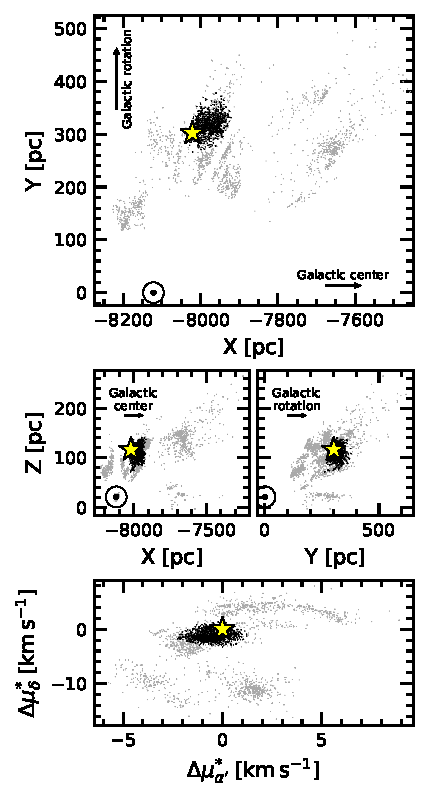
\includegraphics[width=1\textwidth]{f1.pdf}
	\end{center}
	\vspace{-0.7cm}
	\caption{
		{\bf Galactic position and tangential velocities of the
			$\delta$\,Lyr cluster (also known as Theia 73 and Stephenson\,1).}  Points are
		candidate cluster members with $\varpi/\sigma_\varpi > 20$, reported
		to be in the group by \citet{kounkel_untangling_2019}.  We focus
		on stars in a small region (black points) in the kinematic
		vicinity of Kepler\,1627 (yellow star).  The other candidate cluster
		members (gray points) may or may not share the ages of the selected
		kinematic group.  The location of the Sun is ($\odot$) is shown.
		\label{fig:XYZvtang}
	}
\end{figure*}

Figure~\ref{fig:XYZvtang} shows members of the \cn\
reported
by \citet{kounkel_untangling_2019} to be in the group.
Galactic positions are determined and plotted only for stars with parallax
signal-to-noise exceeding 20.
The location of the Sun is shown on the plots.
The non-uniform ``clumps'' might be
an artifact of the data processing steps performed by \citet{kounkel_untangling_2019}.
We therefore only consider stars in the immediate kinematic group
around \sn. 
The tangential velocities relative to \sn\ are shown in the bottom right panel.
These are computed by assuming that every star has the same three-dimensional
spatial velocity as \sn, where we assume a systemic radial velocity of
$-16.7 \pm 0.2$\,\kms\ based on the reconnaissance spectra obtained by
A.~Howard on HIRES and D.~Latham on TRES.
The relevant projection effects are then taken into account,
as discussed by {\it e.g.}, \citet{Meingast2021} and {\bf L.~Bouma et al (2021, submitted)}.

\section{Transit and Stellar Variability Model}
\label{app:gptransit}

We assumed a quadratic limb-darkening law, with the uninformative prior
advocated by CITET Kipping2013.

% In the first approach, we adopted uniform priors centered on the
% interpolated CITET Claret+2011 coefficients in the Kepler-band, with
% with $\pm 0.2$ in either parameter.  The fit was not as good.

Our default stellar variability model (RotGPtransit) allows for a
\texttt{RotTerm} GP kernel, with a logjitter term to inflate the
uncertainties to account for excess white noise.
(This results in an inflation of the uncertainties by a factor
of about three).

We considered including an additive \texttt{SHOTerm} kernel to account
for stochastic noise (RotStochGPtransit).  This didn't seem to affect the results much, so
we opted for the simpler model.



Figure~\ref{fig:phasefold} shows X, Y, Z.  The residuals during the
transit may hint at some small degree of unfitted signal -- in the
sense that the observations are systematically high in the first half
of transit, and low in the second half.  
One possible explanation could be that we are seeing the effects of
gravity darkening (e.g., CITE Masuda 2015).
The expected amplitude of the effect is XXX, based on CITE.
However, there is also a dip of comparable amplitude shortly before
the transit. 
Given the uncertainties in the stellar variability model, we expect
that these patterns may correspond to more noise than signal.

\section{Flare Analysis}
\label{app:flare}

\begin{figure*}[t]
	\begin{center}
		\leavevmode
		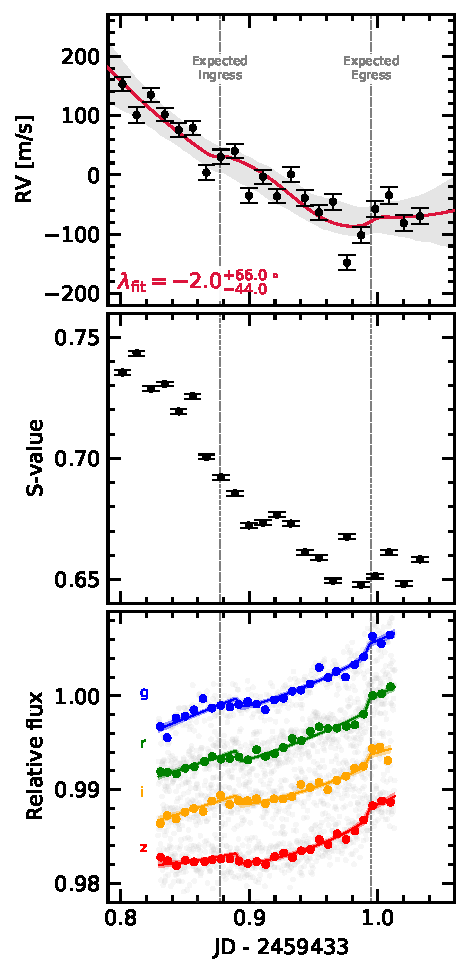
\includegraphics[width=1\textwidth]{f7.pdf}
	\end{center}
	\vspace{-0.7cm}
	\caption{
		{\bf Flares in Kepler\,1627}.  
    {\it Top:}
    The full short-cadence Kepler dataset, acquired at 1-minute
    sampling (black points) is shown with a stellar variability model
    (blue line).
    {\it Middle:}
    Residual after subtracting the stellar variability model.  Flares
    appear as spikes.
    {\it Bottom:}
    Zooms of the brightest, and third-brightest flares.  A timing
    coincidence -- that both flares has ``successors'' approximately
    one orbital period after the initial event -- is emphasized.
		\label{fig:flarezoom}
	}
\end{figure*}

\begin{figure*}[t]
	\begin{center}
		\leavevmode
		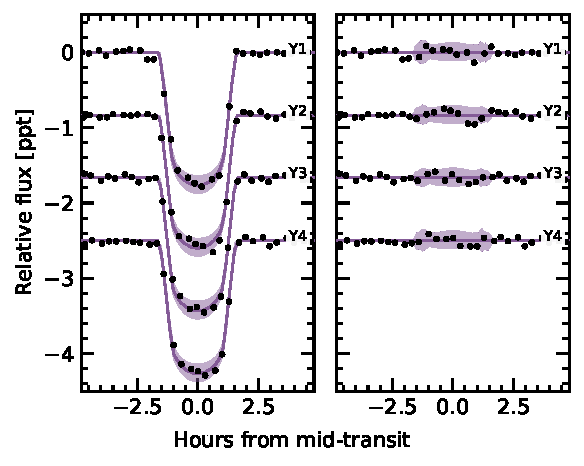
\includegraphics[width=1.0\textwidth]{f8.pdf}
	\end{center}
	\vspace{-0.7cm}
	\caption{
		{\bf Phase-folded flares in Kepler\,1627}.  
    {\it Top:}
    As in the middle of Figure~\ref{fig:flarezoom}, phase-folded at
    the planet's ephemeris.
    {\it Bottom:}
    Fitted flare amplitudes and orbital phases.
    Colors indiate relative time, from the beginning of the
    98-day short-cadence Q15 dataset (dark blue) to the end (light
    yellow).
    Lower amplitude flares likely exist in the data, and were not
    examined.
		\label{fig:flarephase}
	}
\end{figure*}


The 1-minute cadence Kepler observations span 98 days, and cover 24
flares exceeding $0.5\%$ in relative flux.  These 24 flares spanned a
total of 6.5 hours ($\sim$15 minutes per flare).  The coincidence is
that despite the low flare duty cycle, one orbital period after the
the brightest flare, a second flare followed.  This and a similar
event are shown in Figure~\ref{fig:flarezoom}.  The timing error is
good to a $\approx0.2\%$ difference from the orbital period, which
seems {\it a priori} unlikely.  If we consider flares falling within
2\% of the planet's orbital period after a previous flare, then 4 of
the 24 flare events have candidate ``successors''.

A brief note on how we cleaned the light curve, and identified the
flares.
For cleaning, we performed the following iterative detrending procedure.
\begin{itemize}
  \item Step 1: Build a two-term mixed SHOTerm GP model with
    quasi-periodic kernels at Prot and 0.5$\times$Prot. Fit the model
    to the time, flux, and flux uncertainty.
  \item Step 2: Select points more than twice the median absolute
    deviation from the residual, and exclude them from the light
    curve.  Repeat Step 1.
  \item Step 3: On the residual from Step 2, identify all flares,
    requiring them to be at least 20 cadences apart, at least 7 median
    absolute deviations above the median baseline, and lasting at least
    2 cadences in duration.  Build the mask spanning these times, from
    5 minutes before each flare begins to 2.5 minutes after the final
    flare cadence.  Repeat Step 1 a final time.
\end{itemize}

The flares were identified and fitted using ALTAIPONY (CITE CITE).
The fitted model is that of CITE XXX, which parametrizes the flare
with a start time, a lag time, and an amplitude (CHECK).
Figure~\ref{fig:flarephase} shows the resulting flares, amplitudes,
and phases.

We considered two hypotheses: {\it i)} the flare arrival times are
distributed as a Poisson process, and {\it ii)} they are better
explained as a Poisson process with a periodic mixture component.

TODO: explore!  Fit the flare inter-arrival times...
[even the 2-separated ones?]





\section{Companion Star and False Positive Assessment}
\label{app:companionstar}

\begin{figure*}[t]
	\begin{center}
		\leavevmode
		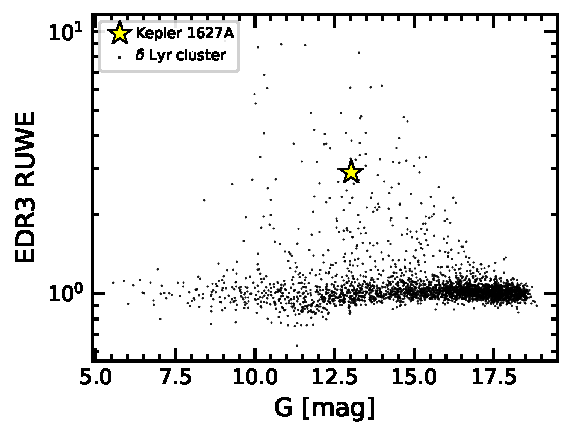
\includegraphics[width=0.6\textwidth]{f6.pdf}
	\end{center}
	\vspace{-0.7cm}
	\caption{
    {\bf Gaia EDR3 renormalized unit weight error (RUWE) point
    estimates for Kepler\,1627A and other members of
    the $\delta$\,Lyr cluster.}  Since other members of the cluster
    with similar colors have comparable degrees of photometric
    variability, the high RUWE estimate suggests that Kepler\,1627A is
    a binary. 
		\label{fig:ruwe}
	}
\end{figure*}

\begin{figure*}[t]
	\begin{center}
		\leavevmode
		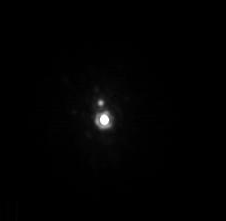
\includegraphics[width=0.6\textwidth]{TEMP_binarity_ao.png}
	\end{center}
	\vspace{-0.7cm}
	\caption{
    {\bf Keck NIRC2 AO image of Kepler 1627A and Kepler 1627B.}  
    {\bf SCALEBAR DENOTES...}
    {\bf North is up, East is left}.
    \label{fig:ao}
	}
\end{figure*}

Our analysis of archival Keck-NIRC2 Kp-band (2.12\,$\mu $m) imaging
revealed the existence of a previously unreported stellar neighbor,
unresolved in the Gaia source catalog {\bf FIXME: uncertainties}.  The
NIRC2 images yield a projected separation $\rho=0\farcs17$, with
$\Delta {\rm Kp} = 2.5$.  Using the measured Gaia EDR3 parallax for
the system, this implies a projected separation of 54\,AU.  The
presence of this star is consistent with the excess noise in the Gaia
astrometric time-series (see Section~\ref{app:companionstar}).  Given
the low chance of a star imaged within {\bf X.X arcseconds} to be a
chance companion along the line of sight, we proceed under the
assumption that it is bound, and that the Kepler\,1627 system is
binary.

Unforuntately, we do not have any reliable color information about
Kepler\,1627B.  Based on the
tabulation\footnote{\url{http://www.pas.rochester.edu/~emamajek/EEM_dwarf_UBVIJHK_colors_Teff.txt},
version \texttt{2021/03/02}.} by \citet{pecaut_mamajek_2013}, the
measured NIR-contrast for a main sequence G8V star corresponds to a
spectral type for the companion of $\approx$M2V ($M_\star \approx
0.44\,M_\odot$).  However, the companion should have a longer
pre-main-sequence contraction phase than the primary, which would
imply that this mass is overestimated by $\sim10$ to $20\%$.

Could the companion be creating a false positive signal?  The
companion star contributes $\approx$1\% of the total flux observed in
the Kepler aperture (0.7-2.0\% V-band to G-band dmag difference from
EEM table; todo is fix using model spectra).  The observed transit has
a depth of 0.18\%.  An 18\% deep eclipse of the secondary star would
therefore be needed to produce a deep enough signal.  The shape of the
observed signal requires allowed impact parameters to span 0.02 to
0.73 (Table~\ref{tab:posterior}); the body transiting the secondary
would therefore need to be non-grazing with $R_3/R_2 \approx 0.42$.
Assuming a $\approx 0.42R_\odot$ radius of the imaged secondary, this
would imply a tertiary stellar radius of $\approx 0.2R_\odot$.  This
scenario ultimately yields a contradiction, because it would require
an ingress and egress phase that each span $\approx$40\% of the
transit duration ($\approx 65\,{\rm minutes}$).  The actual measured
ingress and egress duration is $\approx 15\,{\rm minutes}$),
4.4$\times$ shorter.

\paragraph{Stellar density implied by transit duration}
The duration of the transit ($2.823 \pm 0.057 hr$) and the implied
stellar density ($2.31 \pm 0.52\,{\rm g\,cm}^{-3}$) could in theory
help rule between whether the transiting body orbits the primary or
secondary star.  Ultimately, our stellar density measurement is not
precise enough to render the blend scenario implausible.  At 30 Myr, a
0.40\,$M_\odot$ solar-metallicity dwarf is $\approx 26\%$ larger than
when it is fully contracted on the main sequence (0.40\,$R_\odot$
vs{.} 0.50\,$R_\odot$; CITEALT: Choi et al, MIST grids).  The
theoretically implied companion density of $3.2\,{\rm g\,cm}^{-3}$ is
indeed larger than the primary star's density of $1.80\,{\rm
g\,cm}^{-3}$ (measured through the HIRES reconaissance spectroscopy).
However the stellar density measured from the transit fitting ($2.31
\pm 0.52\,{\rm g\,cm}^{-3}$) is only discrepant at the
$\approx$2-$\sigma$ level from the M-dwarf blend scenario.  It is
instead the combination of the flux contrast, transit depth, and
ingress duration that rule out this scenario.









% \section{Bonus figures that wont be included}
% 
% \begin{figure*}[t]
% 	\begin{center}
% 		\leavevmode
% 		\includegraphics[width=1\textwidth]{dontinclude0.png}
% 	\end{center}
% 	\vspace{-0.7cm}
% 	\caption{
%     {\bf corner plot of gptransit fit}
% 	}
% \end{figure*}


\listofchanges

%\allauthors
\end{document}
